\chapter{Foundations}
\label{sec:foundations}
Firstly, a description of basic but significant architectures that are used in this thesis. Starting by convolutions and then describing more complex architectures like the UNET in section \ref{sec:unet}. Next, the main generative approach explored in this thesis, the Denoising Diffusion Probabilistic Model, will be described. A rough overview of the statistical and visual metrics that were used to evaluate the results in section \ref{sec:results} are given. Finally, discussions about the topic of Continual Learning and how it is defined.
\section{Convolutions}
\label{sec:convolutions}
The principals of Convolutional Neural Networks (CNN) were first described by Fukushima in \cite{Fukushima1980NeocognitronAS}. The name CNN was not set by the time the article was released,
but the idea is used today in many models is still the same. A CNN is a type of neural network designed to process visual or spacial inputs, e.g. images, videos, audio signals or even time series. \newline
A CNN consists of one or more convolutional layers.
A convolutional layer is described as a layer that performs mathematical operations on the input.Those are called convolutions. Convolutions combine the input data with a given set of
filters or kernels, that can be described as specially weighted matrices that are capable of detecting specific features or patterns in the given data. Those features can be edges, corners, different colors, textures or shapes.
This operation is performed by sliding the kernel over the input data and computing the dot product between the kernel and the exposed area of the data as seen in figure \ref{fig:cnn dot}
\begin{figure}
    \centering
    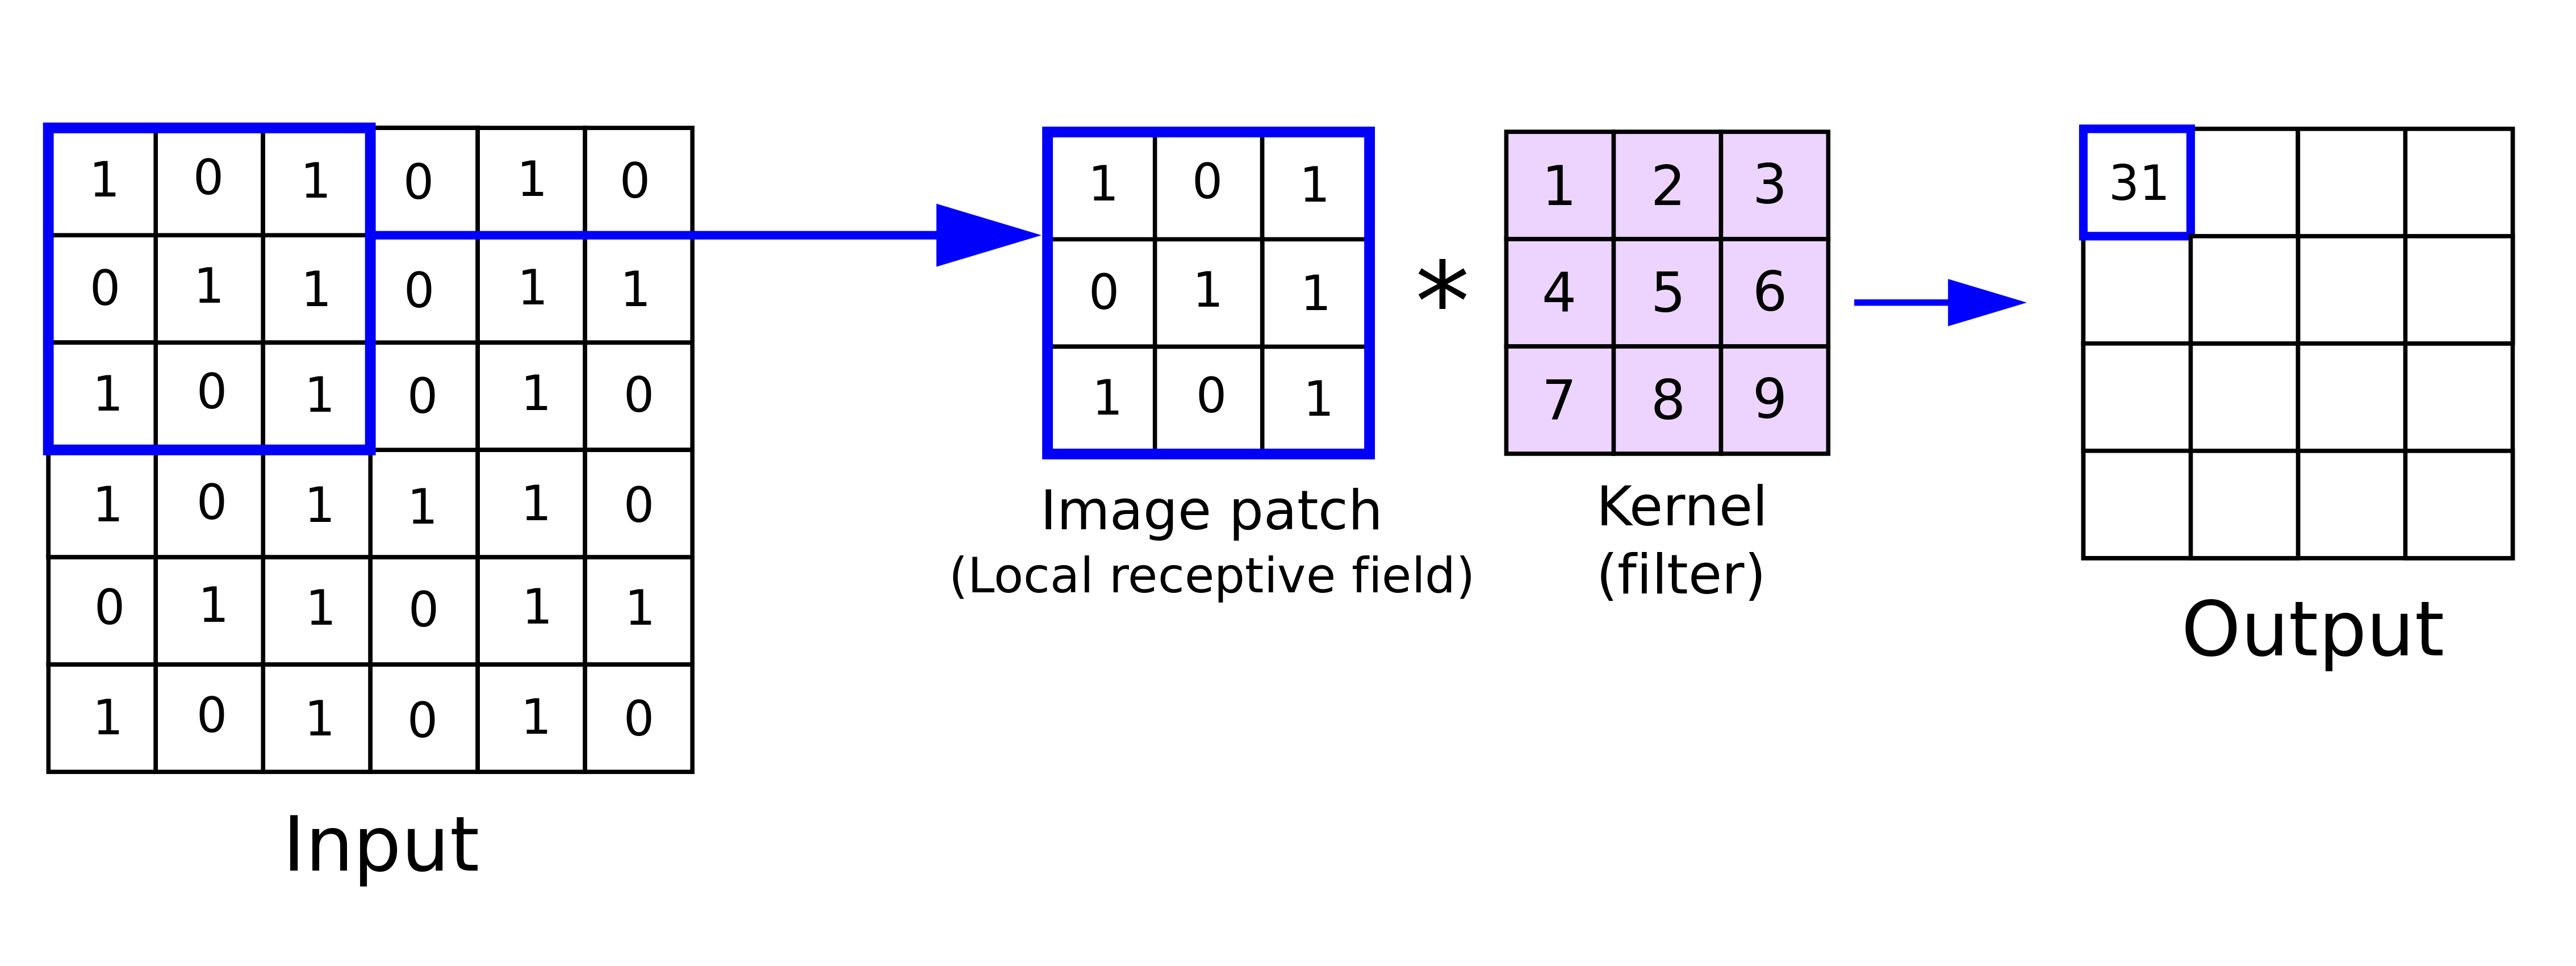
\includegraphics[width=0.85\textwidth]{images/cnn-dot.png}
    \caption{A visualization of a convolutional operation}
    \label{fig:cnn dot}
\end{figure}
\section{UNET}
\label{sec:unet}
The UNET was introduced to tackle the task of image segmentation \cite{ronneberger_unet}. Not an easy task to solve, as it requires 
both high-level semantic information and low-level spatial information of the image.
Traditional convolutional neural networks are good at extracting semantic features, but they tend to lose spatial information due to pooling 
and striding operations that reduce the resolution of the feature maps.
To address this issue, a powerful deep learning architecture called UNET was proposed by Ronneberger et al. in 2015 . 
UNET is based on the idea of Fully Convolutional Networks (FCN), which use only convolutional layers to perform end-to-end 
image segmentation without any fully connected layers. \newline
\begin{figure}
    \centering
    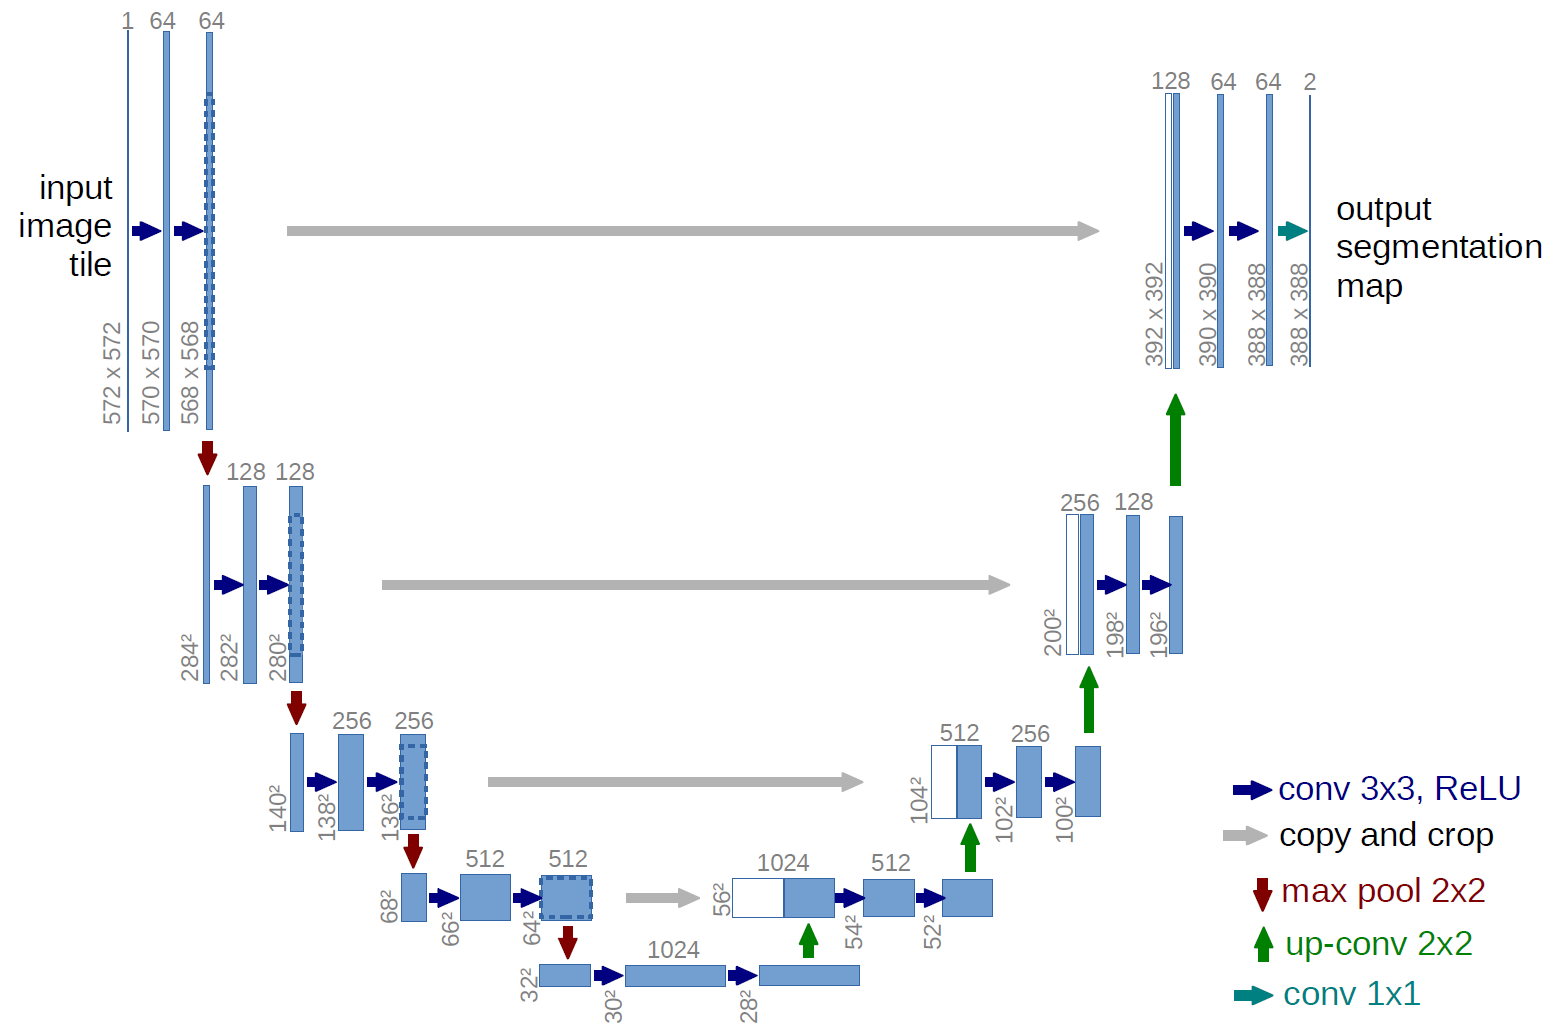
\includegraphics[width=0.85\textwidth]{images/u-net-architecture.png}
    \caption{A graphical visualization of the UNET architecture that was proposed in \cite{ronneberger_unet}.}
    \label{fig:unet}
\end{figure}
The UNET architecture consists of two parts: an encoder and a decoder, as shown in figure \ref{fig:unet}. 
The encoder follows the typical structure of a CNN, with repeated blocks of two 3x3 convolutions followed by 
a Rectified Linear Unit (ReLU) and a 2x2 max pooling operation with stride 2 for downsampling. At each 
downsampling step, the number of feature channels is doubled. \newline
The decoder is symmetric to the encoder, with repeated blocks of two 3x3 convolutions followed by a ReLU and 
a 2x2 up-convolution that halves the number of feature channels and upsamples the feature maps. The up-convolution is implemented by a 
transposed convolution or a bilinear interpolation followed by a 1x1 convolution.
One of the key features of UNET is the skip connections that connect the corresponding layers in the encoder 
and the decoder. These skip connections allow the decoder to use both high-level semantic features and 
low-level spatial features from the encoder, which helps to preserve the fine-grained details of the image 
and improve the segmentation accuracy.\newline
The final layer of UNET is a 1x1 convolution that maps each feature vector to the desired number of classes.
\section{Denoising Diffusion Probabilistic Model}
\label{sec:ddpm}
First, the intuition will be described, followed by the formal definition of a diffusion model. A diffusion probabilistic model or short "diffusion model" is described as a parameterized Markov chain \cite{ho_denoising_2020}. It is trained using variational interference. The goal is to produce matching data samples after a finite time. Starting with noise $x_\mathrm{T}$ the model produces less and less noisy samples $x_\mathrm{T-1} , x_\mathrm{T-2} , ...$. The end of this process results in an authentic sample $x_\mathrm{0}$. Each $t \in [0,T]$ resembles a timestamp that describes a certain noise-image-ratio for an image $x_\mathrm{0}$ and a noise $\epsilon$.  A diffusion model learns to synthesis less noised samples $x_\mathrm{t-1}$ from $x_\mathrm{t}$ by predicting the noise component of $x_\mathrm{t}$. This model is parameterized in \cite{ho_denoising_2020} as function $\epsilon_\mathrm{\theta}(x_\mathrm{t}, t)$.
\begin{figure}
    \centering
    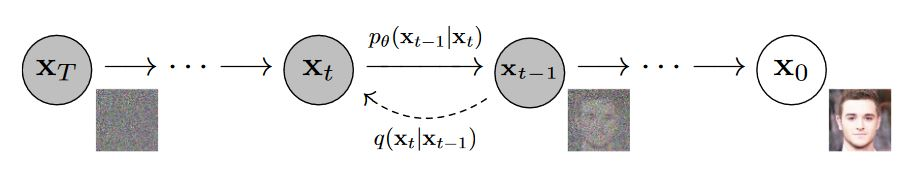
\includegraphics[width=\textwidth]{images/ddpm.JPG}
    \caption{A graphical representation of the noising- and denoising-process.}
    \label{fig:ddpm}
\end{figure}
Training this model is achieved by randomly fetching a data sample $x_\mathrm{0}$, a random timestamp $t$ and a noise $\epsilon$. \newline These result in $x_\mathrm{t}$ using formula \ref{eq:1}, presented in \cite{ho_denoising_2020}. $\beta_\mathrm{t}$ represents a variance schedule that describes the Gaussian noise added to $x_\mathrm{0}$ for $t \in [0,T]$.
\begin{equation}
\label{eq:1}
    q(x_\mathrm{t}|x_{t-1}) = \mathcal{N}(x_\mathrm{t};\sqrt{1-\beta_\mathrm{t}}x_\mathrm{t-1},\beta_\mathrm{t}\mathrm{I}).
\end{equation}
Instead of gradually adding noise over time 1 to T $q(x_\mathrm{t}|x_0)$ can be expressed as a Gaussian distribution with $\alpha:= 1-\beta_\mathrm{t}$ and $\overline{\alpha}_\mathrm{t} := \prod_\mathrm{s=0}^\mathrm{t} \alpha_\mathrm{s}$. The new formula that forms is

\begin{equation}
\label{eq:2}
    q(x_\mathrm{t}|x_0) = \mathcal{N}(x_\mathrm{t};\sqrt{\overline{\alpha}_\mathrm{t}}x_0,(1-\overline{\alpha}_\mathrm{t})\mathrm{I}) \newline 
\end{equation}
\begin{equation}
\label{eq:3}
        = \sqrt{\overline{\alpha}_\mathrm{t}}x_0 + \epsilon\sqrt{1-\overline{\alpha}_\mathrm{t}}, \epsilon\sim \mathcal{N}(0,\mathrm{I}).
\end{equation}
The objective of the training is a simple mean-squared error ${\|\epsilon_\theta(x_\mathrm{t},t)-\epsilon\|}^2$ minimization between the true noise and the predicted noise of the model.\newline \noindent Using the noise predictor $\epsilon_{\theta}(x_\mathrm{t}, t)$ sampling can be achieved. Sampling with a diffusion model is a repeated prediction of $x_\mathrm{t-1}$ from $x_\mathrm{t}$, starting at a randomly initialized $x_\mathrm{T}$. Under reasonable assumptions, using the Bayes theorem, the posterior $q(x_\mathrm{t-1}|x_\mathrm{t},x_0)$ is also a Gaussian with mean-function $\tilde{\mu}(x_\mathrm{t},x_0)$ and fixed variance $\tilde{\beta}_\mathrm{t}$ \cite{nichol_improved_2021}. 
\begin{equation}
\label{eq:4}
    \tilde{\mu}(x_\mathrm{t},x_0):= \frac{\sqrt{\overline{\alpha}_\mathrm{t-1}}\beta_\mathrm{t}}{1-\overline{\alpha}_\mathrm{t}}x_0 + \frac{\sqrt{\alpha_\mathrm{t}}(1-\overline{\alpha}_\mathrm{t-1})}{1-\overline{\alpha}_\mathrm{t}}x_\mathrm{t}
\end{equation}
\begin{equation}
\label{eq:5}
    \tilde{\beta}_\mathrm{t} := \frac{1-\overline{\alpha}_\mathrm{t-1}}{1-\overline{\alpha}_\mathrm{t}}\beta_\mathrm{t}
\end{equation}
\begin{equation}
\label{eq:6}
    q(x_\mathrm{t-1}|x_\mathrm{t},x_0) = \mathcal{N}(x_\mathrm{t-1}; \tilde{\mu}(x_\mathrm{t},x_0),\tilde{\beta}_\mathrm{t}\mathrm{I})
\end{equation}
Theoretically, sampling from $q(x_0)$ works by first sampling from $q(x_\mathrm{T})$ and then sample the reverse steps $q(x_\mathrm{t-1}|x_\mathrm{t})$ until $x_0$ is reached. Reasonable settings for $\beta_\mathrm{t}$ and \(T\) provide trivial sampling for $x_\mathrm{T}$, because the distribution $q(x_\mathrm{T})$ is nearly an isotropic Gaussian distribution \cite{dhariwal_diffusion_2021}.\newline \noindent
After establishing all necessary steps, an approximation of $q(x_\mathrm{t-1}|x_\mathrm{t})$ is missing. Using a neural network to predict mean $\mu_\theta$ and a diagonal covariance matrix $\Sigma_\theta$ is considered. This is possible because \cite{sohl-dickstein_deep_2015} notes that the distribution $q(x_\mathrm{t-1}|x_\mathrm{t})$ approaches a diagonal Gaussian distribution for $T \rightarrow \infty$, which corresponds to $\beta_\mathrm{t} \rightarrow 0$.
\begin{equation}
\label{eq:7}
    p_\theta(x_\mathrm{t-1}|x_\mathrm{t}) := \mathcal{N}(x_\mathrm{t-1};\mu_\theta(x_\mathrm{t},t),\Sigma_\theta(x_\mathrm{t},t))
\end{equation}
The model goal is to learn the true data distribution $q(x_0)$. In \cite{ho_denoising_2020} it is shown that a different objective produces better samples in general. Therefore they don't directly predict $\mu_\theta(x_\mathrm{t},t)$ with a neural network, but rather $\epsilon_{\theta}(x_\mathrm{t}, t)$ so it matches the noise $\epsilon$  used in \ref{eq:3}. During the sampling process, $\mu_\theta(x_\mathrm{t},t)$ can be derived from $\epsilon_{\theta}(x_\mathrm{t}, t)$ by substitution:
\begin{equation}
\label{eq:8}
    \mu_\theta(x_\mathrm{t},t) = \frac{1}{\sqrt{\alpha_\mathrm{t}}}\left(x_\mathrm{t} - \frac{1-\alpha_\mathrm{t}}{\sqrt{1-\overline{\alpha}_\mathrm{t}}}\epsilon_{\theta}(x,t)\right)
\end{equation}
This mathematical foundations are put to use at different data structures to create generative models. The following chapters contain two contexts of generative models using DDPMs.
\newpage
\section{Maximum Mean Discrepancy}
\label{sec:mmd}
The maximum mean discrepancy (MMD) \cite{gretton2008kernel} is a statistical indicator that can be used to determine how close to each other underlying sample distributions are.
A small MMD indicates high similarity. This can be used in generative models to compare synthetic sample sets with real sample sets.
Decent MMD scores can so be used to argue that models perform good in the the task of synthesizing the real data distribution.\newline
In practice, the squared difference between the two sets is considered as presented in \cite{esteban2017realvalued}.
The assumptions that they introduce and the operations that are performed result in a score that can be used to estimate the quality of 
a generative model.\newline \newline
\resizebox{\textwidth}{!}{$\widehat{\textbf{MMD}}^{2} = \frac{1}{n(n-1)}\sum_{i=1}^{n}\sum_{j\neq i}^{n}K(x_{i},x_{j})-
\frac{2}{mn}\sum_{i=1}^{n}\sum_{j= 1}^{m}K(x_{i},y_{j})+
\frac{1}{m(m-1)}\sum_{i=1}^{m}\sum_{j\neq i}^{m}K(y_{i},y_{j})$} \newline\newline
Where $K:X \times Y \rightarrow \mathbb{R} $ is a given kernel and $\{x_{i}\}^{D_{real}}_{i=1}$,
$\{y_{j}\}^{D_{fake}}_{j=1}$ are real and synthetic samples.
\section{t-SNE}
\label{sec:tsne}
One method used for evaluation is the t-distributed stochastic neighbor embedding (t-SNE), which is employed for visualization proposed in \cite{maaten2008tsne}.
t-SNE is a method that maps high dimensional data samples into a two- or three-dimensional embedding. First it computes probabilities proportional to the similarity of each data points on the high dimensional representation. Afterwards it tries to find lower dimensional representations by minimization of the Kullback-Leibler divergence.\newline
In the end the lower dimensional data points can be visualized in a scatterplot, e.g. seen in \ref{fig:tsne example}.
t-SNE is interesting for this thesis because time series data, in comparison to image data, is not simply evaluated by looking at a time series graph. Having a visualization method holds great benefits for understanding since it tranforms high dimensional time series data into an interpretable representation for humans.
\begin{figure}[h!]
    \centering
    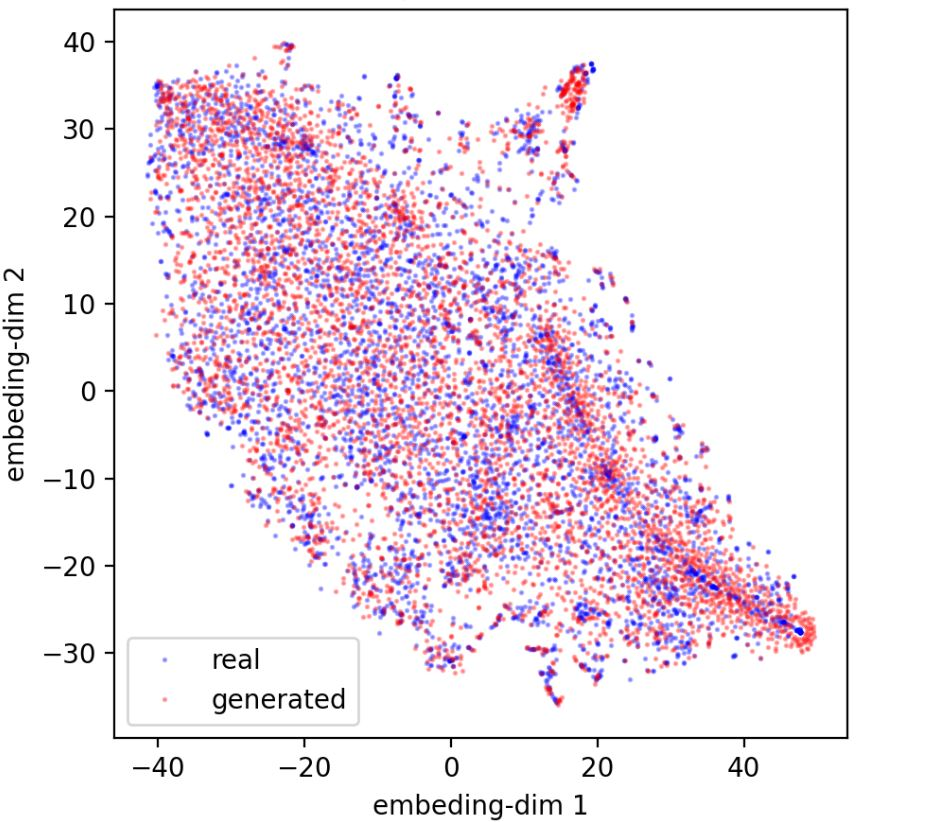
\includegraphics[width=0.75\textwidth]{images/tsne example.JPG}
    \caption{An example of an t-SNE plot where two distributions of time series data were embedded.}
    \label{fig:tsne example}
\end{figure}
\newpage
\section{Continual Learning}
\label{sec:cont learning}
Continual Learning (CL) is the question whether intelligent agents are capable of containing/remembering 
knowledge through different sample distribution that are given to the model iteratively in multiple distinguished training cycles.
It can be described as lifelong training with changing sample distributions which the agent must learn without losing performance on past data distributions.
One effect that occurs during continual learning scenarios is known as catastrophic forgetting \cite{wang2023comprehensive}. 
This term describes a model that is gradually getting worse at older tasks that it learned during its lifetime. To prevent this effect different methods and approaches were investigated. In \cite{wang2023comprehensive} a variety of different CL approaches. Those can be seen in figure \ref{fig:cl_tax}.
\begin{figure}[h!]
    \centering
    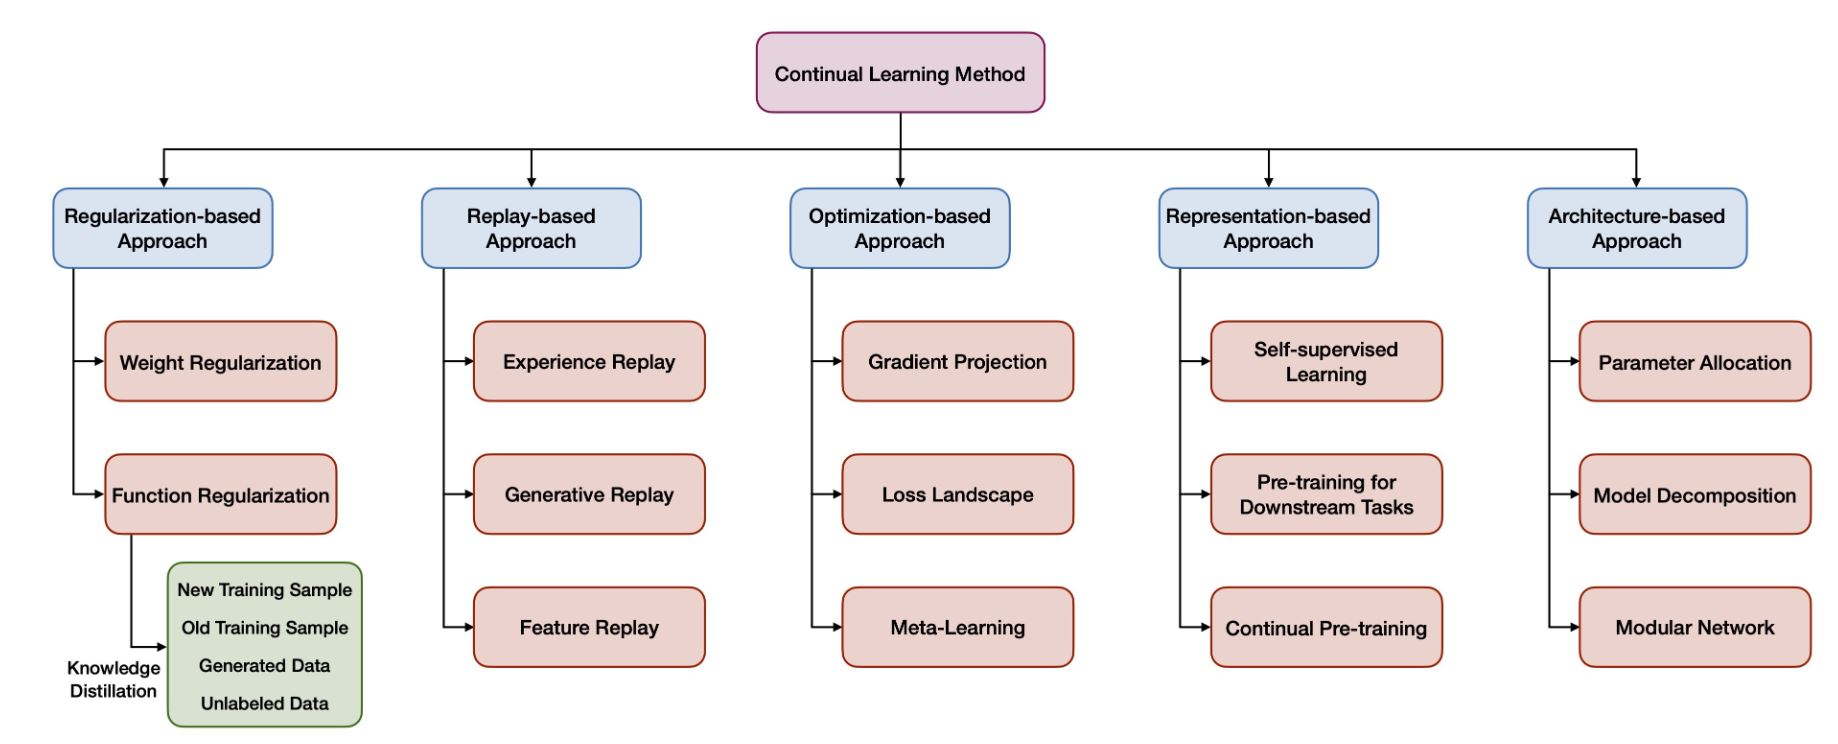
\includegraphics[width=\textwidth]{images/cl_taxonomie.JPG}
    \caption{A state-of-the-art and elaborated taxonomy of representative continual learning methods found in \cite{wang2023comprehensive}.}
    \label{fig:cl_tax}
\end{figure}